%-------------------------------------------------------------------------------
% Definitions
%-------------------------------------------------------------------------------
% here we define authors and titles
%
\providecommand{\theauthorsfull}{Mirko van der Baan} %full list of authors - eg Mirko van der Baan and David Eaton
\providecommand{\theauthorsshort}{Van der Baan} %short list of authors (max 40 characters} - eg Van der Baan and Eaton or Van der Baan et al.
\providecommand{\thetitlefull}{Your full report title comes here}
\providecommand{\thetitleshort}{Your short title} % max 40 characters
%-------------------------------------------------------------------------------
% REPORT SECTION
%-------------------------------------------------------------------------------

\chapter[\theauthorsshort: \thetitlefull]{\thetitlefull \\ \vbox{}
{\LARGE\em  Mirko van der Baan${}^a$ and SomeOne Else${}^b$}\\ %Replace with your own list of authors
\vbox{}
{\small\em 
% place address here
${}^a$ Dept. of Physics, Univ. of Alberta, Edmonton, AB, T6G 2G7, Canada.  E: Mirko.vanderBaan@ualberta.ca \\[-10pt]
${}^b$ Dept. of Physics, Univ. of Alberta, Edmonton, AB, T6G 2G7, Canada.  E: Mirko.vanderBaan@ualberta.ca
}} % don't remove!
%
\rhead[Microseismic Industry Consortium Vol. \thereportvolume\ -- Chapter \thechapter]{\em \thetitleshort}
\lhead[\theauthorsshort]{Microseismic Industry Consortium Vol. \thereportvolume\ -- Chapter \thechapter}

%
\section*{Summary}%\footnote{Paper presented at the 74th EAGE conference, Copenhagen, 2012.}}
%
It is all exciting. Your text comes here. Just replace this short introduction with your actual abstract, but first read these guidelines.

We recommend the use of the MiKTeX installation and TeXstudio or TeXnicCenter as the software to run this template. These two programs are integrated into proTeXt (``proTeXt aims to be an easy-to-install TeX distribution for Windows, based on MiKTeX" \verb"https://www.tug.org/protext/" ). The references are included in this chapter using \verb"bibitem", if you want to use bibtex then read the abstract of the next chapter.

You must  abide by the following schedule:
\begin{itemize}
  \item Oct 21 -- first draft,
  \item Nov 4 -- second draft, and,
  \item Nov 11 -- final version due (no exceptions: if you miss this deadline then you can't publish for a year).
\end{itemize}  

%
\section{Introduction: General rules}
%
Some general rules
\begin{enumerate}
\item Please do not add or remove any packages from \verb"main.tex", but you should rename your folder and your chapter with your own name. 
\item When using cross-referencing to equations, figures and tables make sure you use unique identifiers. 
\item Do not make changes to \verb"main.tex".
\item Do not make changes to \verb"main.tex".
\item Do not make changes to \verb"main.tex". If you do, you have just volunteered to put the entire report together. 
\end{enumerate}

%
\section{Cross-referencing}
%
We are using the cross reference package in this report, so if we want to refer to the convolutional model in (\ref{eq:your_name_convmodel}). In our text we call this equation by \verb"\ref{label}". 

\begin{equation}\label{eq:your_name_convmodel}
s(t) = w(t)\star r(t) + \eta(t).
\end{equation}

Did you know equations are part of sentences so you should use punctuation at the end of each equation?

The same happens referencing Figure \ref{fig:your_name_fig1}. (Use \verb"Figure \ref{label}"). 

If you want to say that \cite{VanderBaan2008} did something then that's ok.
But maybe you prefer to put it as an statement \citep{VanderBaan2008}?

\section{Use figures}

Figures are welcome too, place them in your own folder. In this template you can use different formats (jpg, png, eps or pdf), the compiler will take care of the conversion to pdf. Just call the pdflatex compiler and you will get a nice final pdf document. Use \verb"\begin{figure}" for a figure within a single column and \verb"\begin{figure*}" for a figure spanning two columns.  The same is true for tables.  Use \verb"\begin{table}" for a figure within a single column and \verb"\begin{table*}" for a figure spanning two columns.
%

%
\begin{figure}[htb]
\begin{center}
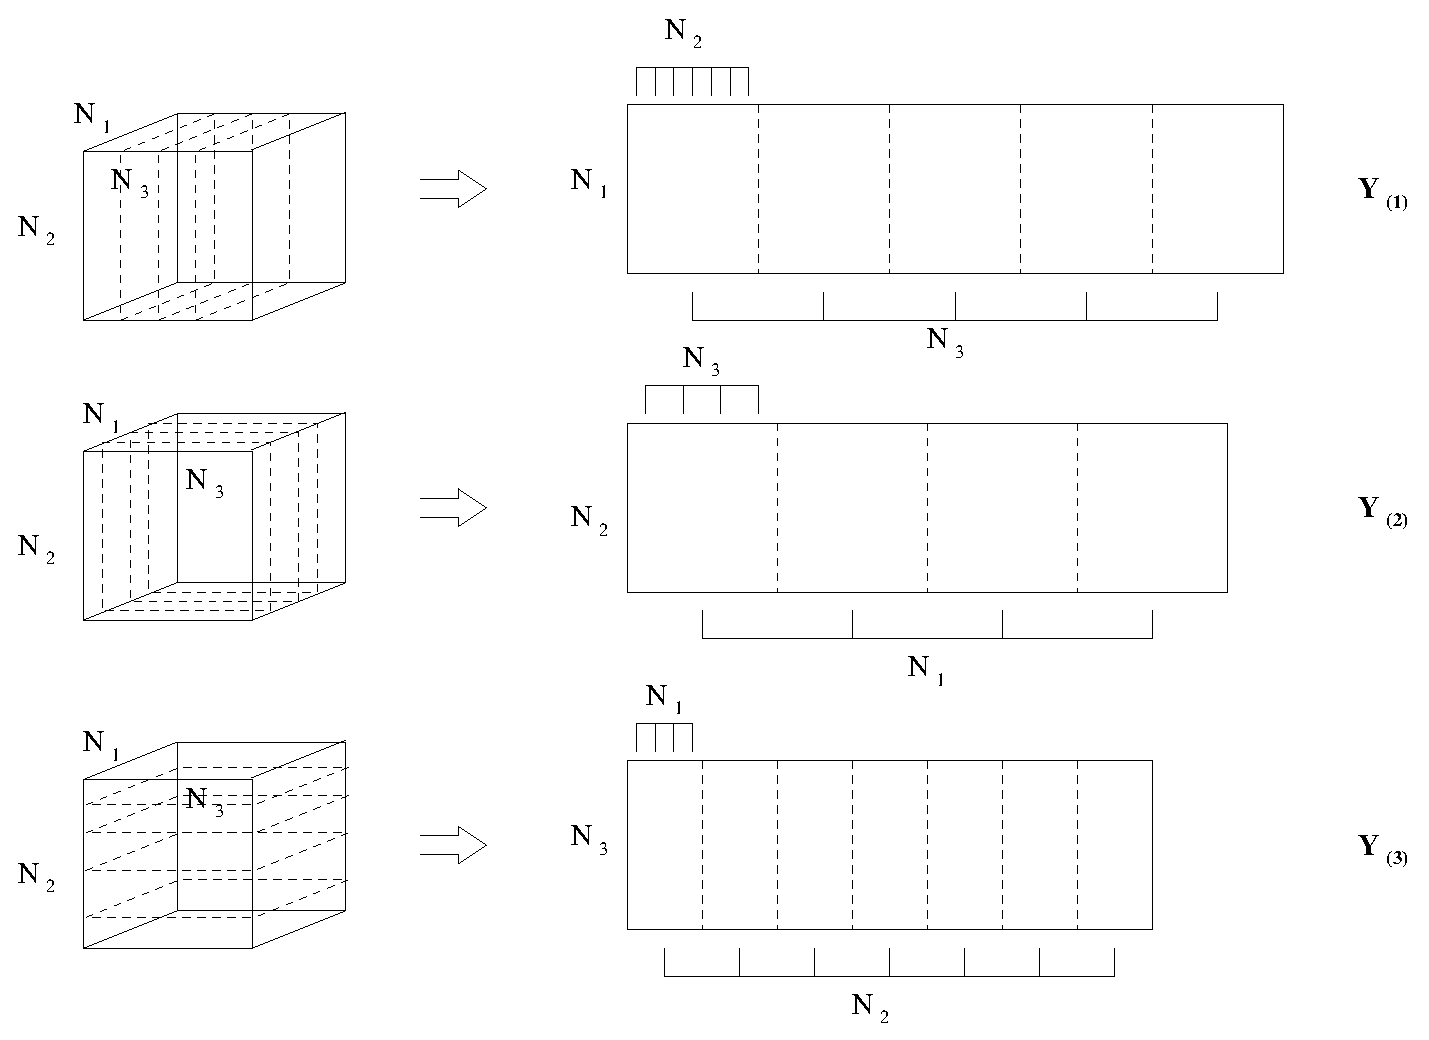
\includegraphics[width=0.7\linewidth,angle=0]{your_chapter_bibitem/fig1.eps}
\end{center}
\vspace{-4mm}
\caption{Your caption}
\label{fig:your_name_fig1}
\end{figure}
%

%
\begin{figure*}[htb]
\begin{center}
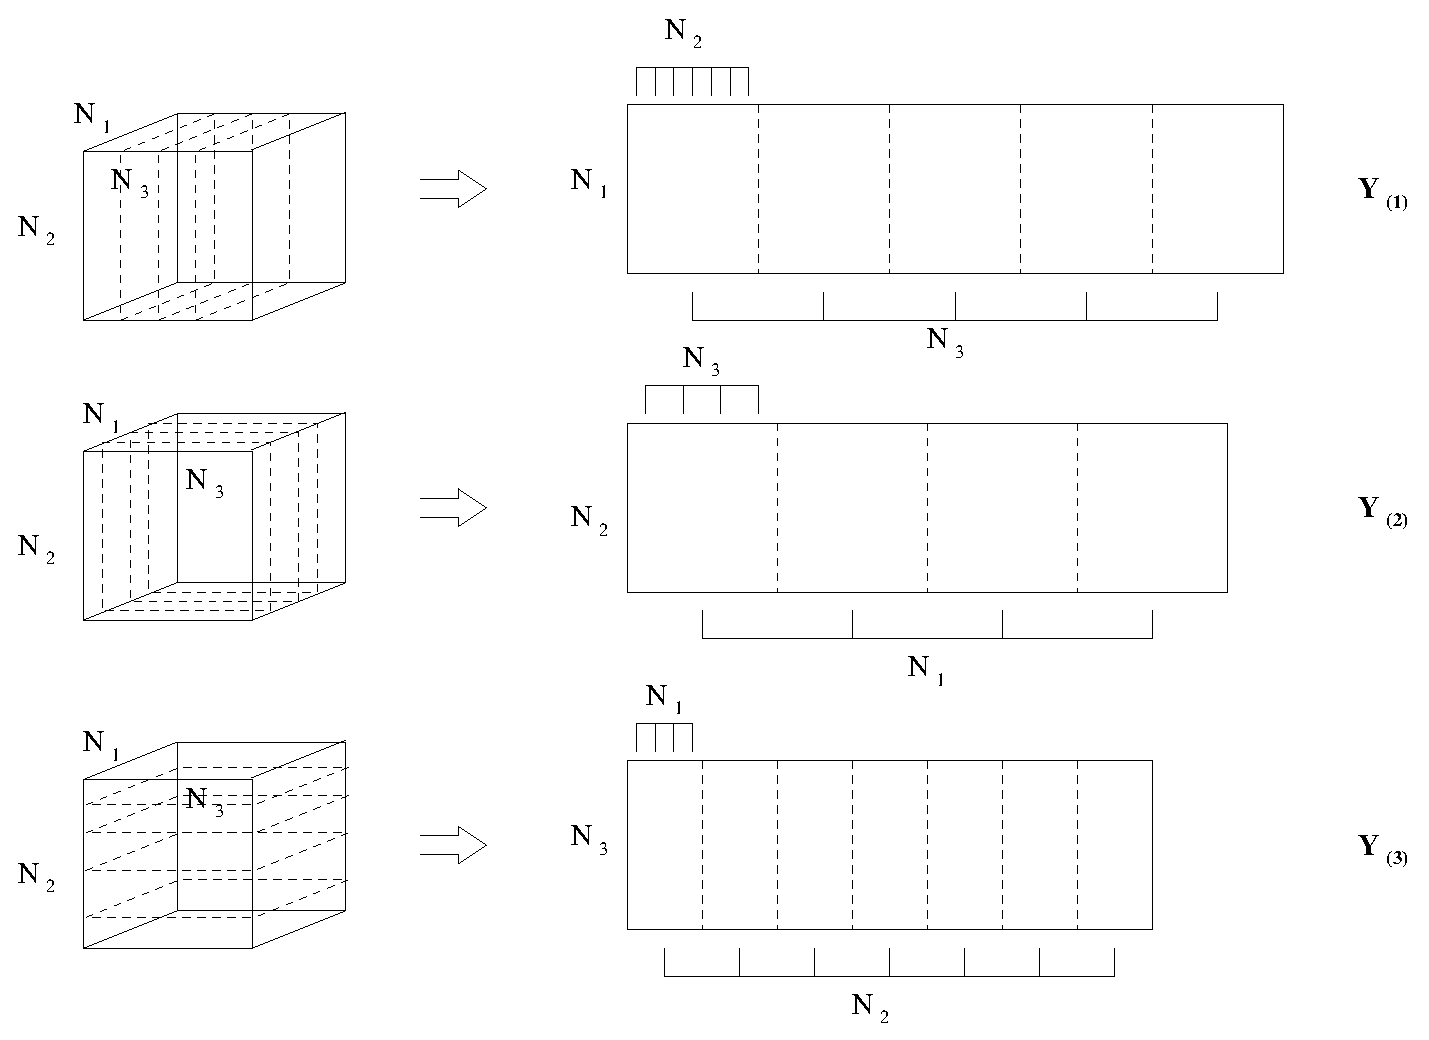
\includegraphics[width=0.7\linewidth,angle=0]{your_chapter_bibitem/fig1.eps}
\end{center}
\vspace{-4mm}
\caption{Your caption}
\label{fig:your_name_fig2}
\end{figure*}
%


%
\section{Acknowledgments}
%
The author would like to thank the sponsors of the Microseismic Industry Consortium for financial support.
%

\begin{thebibliography}{}
\itemsep0pt

\bibitem[Van~der Baan, 2008]{VanderBaan2008}
Van~der Baan, M., 2008, {Time-varying wavelet estimation and deconvolution by
  kurtosis maximization}: Geophysics, {\bf 73}, no. 2, V11-V18.

\end{thebibliography}

